
The central finding is a single pattern that recurs across every capability axis we measured:
biological CPT \emph{lifts} the model, and subsequent SFT \emph{narrows} it back
(Figure~\ref{fig:ucurve}, Figure~\ref{fig:radar}). We present the three completed axes, then the
reasoning-behavior diagnostics.

\begin{figure}[h]\centering
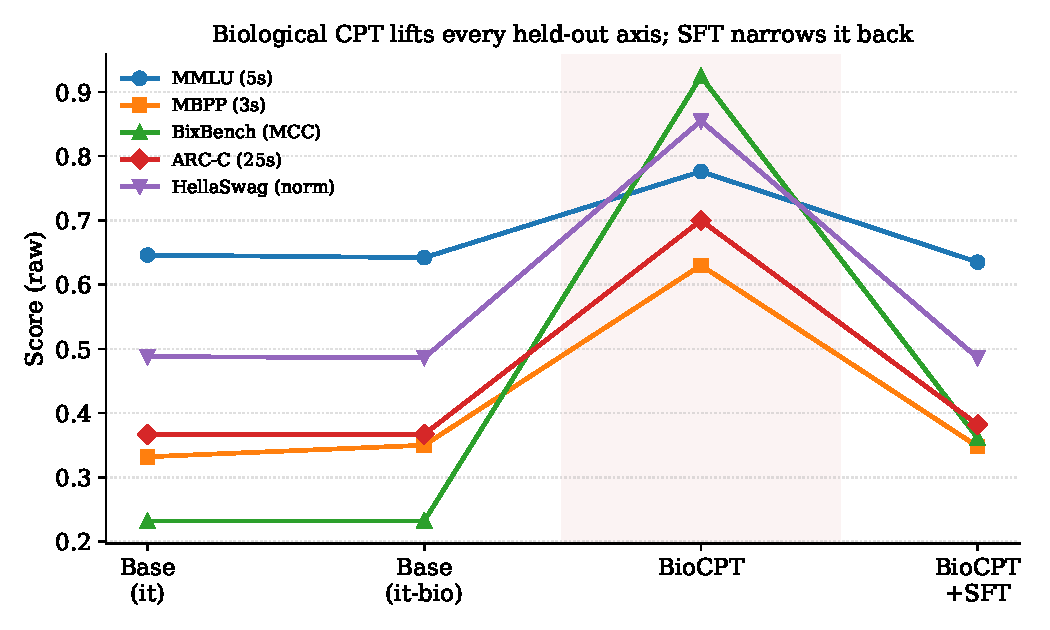
\includegraphics[width=0.82\linewidth]{figs/fig1_ucurve.pdf}
\caption{Every held-out capability axis follows the same trajectory: flat across the
vocabulary-expansion control (it $\to$ it-bio), a sharp rise at biological CPT (shaded), and a
fall back toward base after SFT. Raw scores; see Tables~\ref{tab:general}--\ref{tab:coding}.}
\label{fig:ucurve}
\end{figure}

\subsection{Vocabulary expansion is free}
Before attributing anything to CPT we rule out the tokenizer. The original model (it) and the
vocabulary-expanded but untrained model (it-bio) are indistinguishable on every general
benchmark (MMLU $0.646$ vs.\ $0.642$; ARC-C $0.367$ vs.\ $0.367$; HellaSwag-norm $0.488$ vs.\
$0.486$; TruthfulQA $0.533$ vs.\ $0.532$; all $\le0.4$ pt). Adding $28$K biological tokens to
the vocabulary therefore costs nothing in general competence, and any change at the BioCPT stage
is attributable to the continued pretraining itself.

\subsection{General knowledge and reasoning rise, not fall}
Table~\ref{tab:general} shows the (1) General axis. Against the intuition of catastrophic
forgetting, biological CPT \emph{improves} the model: MMLU $+13.0$ points ($0.646\!\to\!0.776$),
ARC-Challenge accuracy nearly doubles ($0.367\!\to\!0.700$), and HellaSwag-norm rises
$+36.7$ points. The one regression is TruthfulQA ($-8.8$ points), an interpretable drift on
truthfulness/anti-misinformation after heavy exposure to sequence and literature text. We note
honestly that part of the ARC/HellaSwag jump is mechanistic --- an instruction-tuned model is
weak at raw-loglikelihood multiple choice, and CPT on raw text restores base-model-like MC
behavior --- but MMLU ($+13$ pt, knowledge-heavy) is a hard gain unaffected by this. Subsequent
SFT returns all four metrics to near-base levels.

\begin{table}[h]\centering\small
\caption{(1) General. Biological CPT lifts general knowledge/reasoning; SFT narrows it back.
Loglikelihood multiple-choice; community-standard few-shot.}
\label{tab:general}
\begin{tabular}{lccccc}
\toprule
Checkpoint & MMLU (5s) & ARC-C acc (25s) & ARC-C norm & HellaSwag norm (10s) & TruthfulQA-mc2 \\
\midrule
Base (it)        & 0.646 & 0.367 & 0.403 & 0.488 & 0.533 \\
Base (it-bio)    & 0.642 & 0.367 & 0.402 & 0.486 & 0.532 \\
\textbf{BioCPT}  & \textbf{0.776} & \textbf{0.700} & \textbf{0.730} & \textbf{0.855} & 0.445 \\
BioCPT+SFT       & 0.635 & 0.382 & 0.396 & 0.486 & 0.562 \\
\bottomrule
\end{tabular}
\end{table}

\subsection{Code capability nearly doubles}
Code is a structured formal language, and the (3) Coding axis (Table~\ref{tab:coding}) shows the
same shape. On MBPP (3-shot, the format-fair metric), pass@1 rises from $0.33$ at base to
$\mathbf{0.63}$ after BioCPT, then falls to $0.35$ after SFT. (HumanEval 0-shot is excluded:
bare completion is unfair to instruction/SFT checkpoints, which score ${\approx}0$; we report
it only for completeness.) That biological-sequence CPT nearly doubles Python coding ability is
consistent with the hypothesis that structured-sequence pretraining strengthens a shared
substrate for formal/structural languages.

\begin{table}[h]\centering\small
\caption{(3) Coding. MBPP 3-shot is the fair metric (HumanEval 0-shot excluded, see text).}
\label{tab:coding}
\begin{tabular}{lcc}
\toprule
Checkpoint & HumanEval 0s (excl.) & \textbf{MBPP 3s pass@1} \\
\midrule
Base (it)        & 0.012 & 0.332 \\
Base (it-bio)    & 0.000 & 0.350 \\
\textbf{BioCPT}  & 0.439 & \textbf{0.630} \\
BioCPT+SFT       & 0.000 & 0.348 \\
\bottomrule
\end{tabular}
\end{table}

\subsection{Biomedical knowledge: the same curve}
On BixBench (biomedical true/false, loglikelihood-scored MCC), the (2) Biology axis reproduces the
pattern exactly: MCC $0.232$ at base $\to$ $\mathbf{0.924}$ after BioCPT $\to$ $0.361$ after SFT.
Protein sequence-homology, by contrast, is not measurable zero-shot by any simple probe (forced
Yes/No loglikelihood is near-random for all checkpoints; see \S\ref{sec:setup}); we read this as
evidence that sequence-homology ability is \emph{installed into representations} by CPT but only
\emph{cashed out} into task performance by SFT, consistent with prior dual-mode results on this
model family~\citep{wang2026omnigene}.

\subsection{Reasoning behavior: CPT shifts the observable reasoning trajectory}
The three axes above concern \emph{what} the model knows. We finally ask whether CPT changes the
\emph{observable trajectory} of its chain-of-thought generations, independent of accuracy --- a
behavioral phenotype of the output text, not a claim about internal reasoning process. On $200$
GSM8K problems, each sampled $k{=}5$ times under a shared 8-shot chain-of-thought scaffold, we
measure generated chain length, self-correction markers (``wait/actually/however/reconsider''),
hedging markers, and self-consistency (agreement of the final answer across the $5$ samples).
Table~\ref{tab:cot} and Figure~\ref{fig:reasoning} show a striking shift in this observable
phenotype at the BioCPT stage: the generated chain \emph{shortens by 41\%} ($108.8\!\to\!64.4$
tokens) and self-correction markers \emph{nearly vanish} ($0.370\!\to\!0.006$ backtracks per
generation), yet accuracy does not fall (it rises slightly, $0.667\!\to\!0.689$) and
self-consistency is unchanged ($0.745$). Biological CPT --- pretraining on deterministic,
low-redundancy sequence continuation --- appears to shift the model's generated text toward a
\emph{shorter, less self-revising} trajectory. Subsequent SFT reverses this: generated chains
grow past base length ($125.8$ tokens), backtracking and hedging markers return. This is the
same CPT-shapes / SFT-re-shapes signature seen on the knowledge axes, now visible in the
generated reasoning \emph{trajectory} rather than outcome --- a phenotype invisible to accuracy
alone. (it and it-bio again coincide, confirming the clean vocabulary ablation.)

\begin{figure}[h]\centering
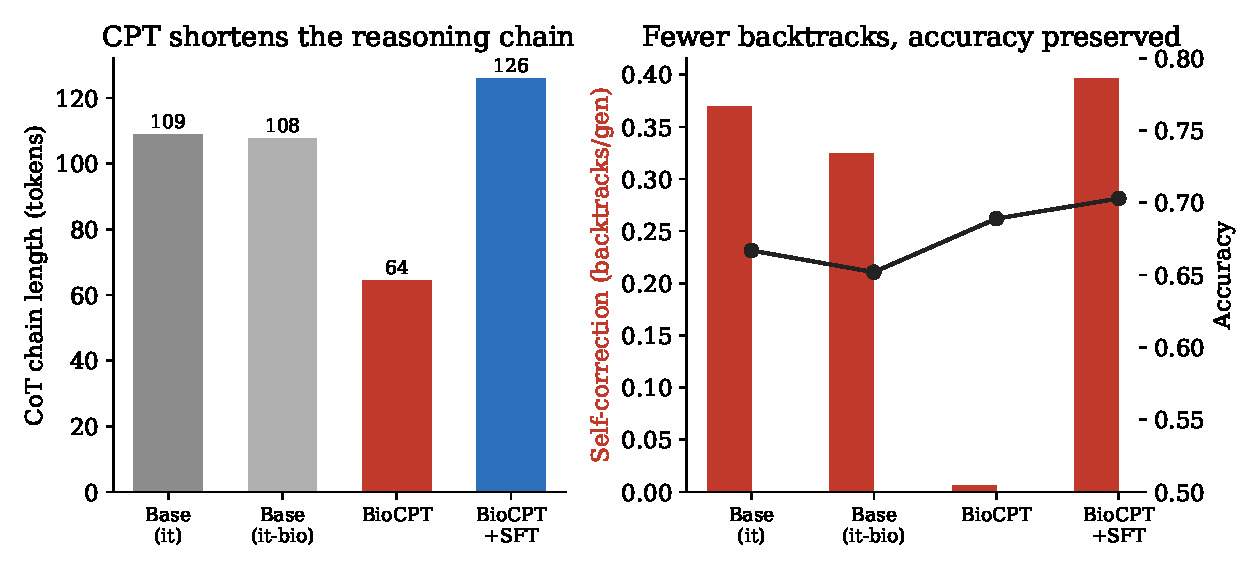
\includegraphics[width=0.92\linewidth]{figs/fig3_reasoning.pdf}
\caption{Observable reasoning-trajectory phenotype on GSM8K. \textbf{Left:} biological CPT
shortens the generated chain-of-thought by 41\%. \textbf{Right:} self-correction markers
(backtracks) nearly vanish at BioCPT while accuracy is preserved (even slightly improved); SFT
reverses both. CPT shifts the generated trajectory toward shorter, less revision-heavy text.}
\label{fig:reasoning}
\end{figure}

\begin{table}[h]\centering\small
\caption{(4) Reasoning-behavior diagnostics on GSM8K (200 questions, $k{=}5$ samples, shared
8-shot CoT). CPT shortens the generated chain and removes self-revision markers without hurting
accuracy; SFT reverses both.}
\label{tab:cot}
\begin{tabular}{lccccc}
\toprule
Checkpoint & Chain len (tok) & Backtrack/gen & Hedge/gen & Self-consist. & Acc.\ (2nd) \\
\midrule
Base (it)        & 108.8 & 0.370 & 0.001 & 0.749 & 0.667 \\
Base (it-bio)    & 107.5 & 0.324 & 0.000 & 0.728 & 0.652 \\
\textbf{BioCPT}  & \textbf{64.4} & \textbf{0.006} & 0.000 & 0.745 & 0.689 \\
BioCPT+SFT       & 125.8 & 0.396 & 0.018 & 0.757 & 0.703 \\
\bottomrule
\end{tabular}
\end{table}

\subsection{Summary}
Across every completed axis the ordering is identical: base $<$ \textbf{BioCPT} $>$ SFT, with
BioCPT the peak (Figure~\ref{fig:radar}). Biological CPT is not a tax; it is an investment in a
shared capability substrate. SFT then trades breadth for task focus.

\begin{figure}[h]\centering
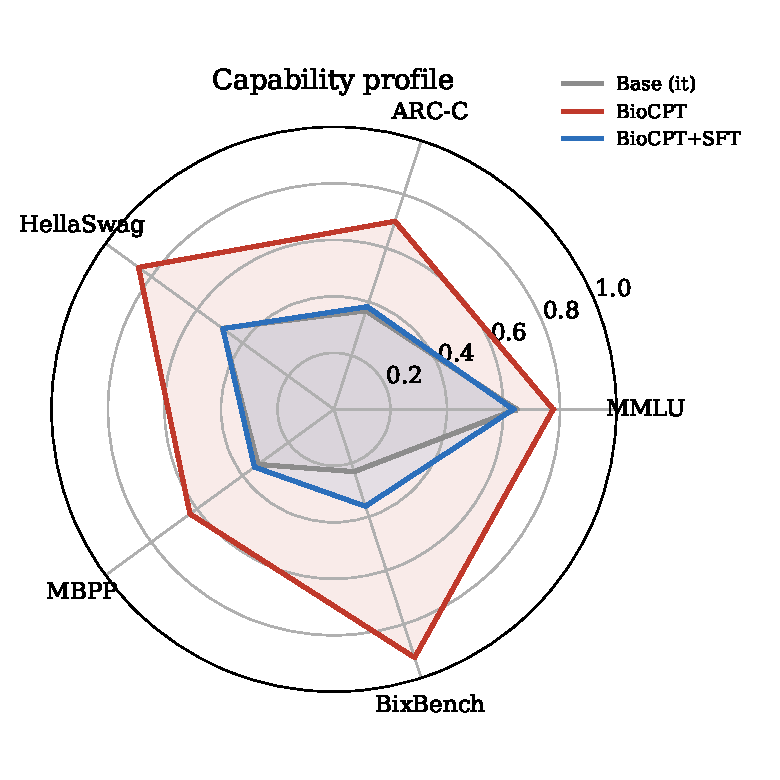
\includegraphics[width=0.60\linewidth]{figs/fig2_radar.pdf}
\caption{Capability profile of the three trained states. BioCPT (red) dominates the base model
on every axis; SFT (blue) retreats toward base on all held-out axes. The biological CPT stage,
not SFT, is what expands the profile.}
\label{fig:radar}
\end{figure}
